\documentclass[11pt]{article}

\usepackage[utf8]{inputenc}
\usepackage{fancyhdr}
\usepackage{hyperref}
\usepackage{graphicx}

\graphicspath{ {images/} }
 
\pagestyle{fancy}
\fancyhf{}
\lhead{University of the Witwatersrand}
\rfoot{School of Computer Science and Applied Mathematics}
\pagenumbering{roman}
\fancyfoot[R]{\thepage}

\begin{document}
\begin{page}

\newcommand{\HRule}{\rule{\linewidth}{0.3mm}} % Defines a new command for the horizontal lines, change thickness here
\renewcommand\section{\@startsection{section}{1}{\z@}%
                                  {-3.5ex \@plus -1ex \@minus -.2ex}%
                                  {2.3ex \@plus.2ex}%
                                  {\normalfont\large\bfseries}}
\setlength{\parindent}{0pt}

\center % Center everything on the page
 
%----------------------------------------------------------------------------------------
%	HEADING SECTIONS
%----------------------------------------------------------------------------------------

\textsc{\LARGE University of the Witwatersrand}\\[1.5cm] % Name of your university/college
\textsc{\Large School of Computer Science and Applied Mathematics}\\[0.5cm] % Major heading such as course name

%----------------------------------------------------------------------------------------
%	TITLE SECTION
%----------------------------------------------------------------------------------------

\HRule \\[0.4cm]
{ \huge \bfseries COMS3008: Parallel Computing Lab Assignment 2}\\[0.4cm] % Title of your document \\
  \large 25 July 2016
\HRule \\[1.5cm]
 
%----------------------------------------------------------------------------------------
%	AUTHOR SECTION
%----------------------------------------------------------------------------------------
\begin{minipage}{1\textwidth}
	\Large \emph By Chalom, J. (711985)\\
\end{minipage}


\vfill % Fill the rest of the page with whitespace

\end{page}

\begin{page}

\clearpage
\setcounter{page}{1}
\pagenumbering{arabic}

\section{Directed Acyclic Graphs}
\noindent \chapter{Chosen Decomposition:} \\
\noindent Let $n$ be the number whose factorial is being investigated. \\
$ n = \{ n \in \mathbb{Z}\ |\ 1 \leq n \leq \mathbb{Z}\} $ 
\\

\begin{figure}[ht]
\centering
     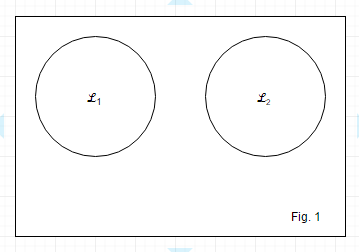
\includegraphics[width=1.0\textwidth]{parallel_fig1}\\
     Data dependency diagram of chosen decomposition
\end{figure}
\noindent Let $L$ be the set of numbers constructed from n such that $L = \{ L \in \mathbb{Z}\ |\ n \leq L \leq 1\}$.
Therefore let $L_1$ and $L_2$ be subsets of $L$ such that $L \in (L_1 + L_2) $.

\noindent Let $L_1$

\begin{figure}[ht]
\centering
     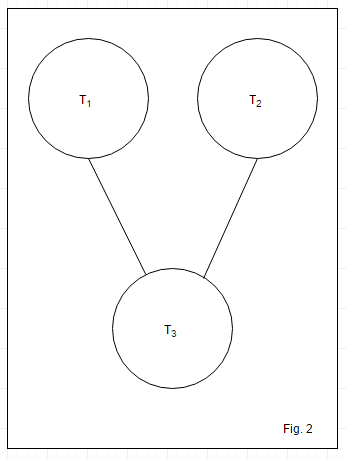
\includegraphics[scale=0.75]{parallel_fig2}\\
     Task interaction diagram of chosen decomposition
\end{figure}

\begin{figure}[ht]
\centering
     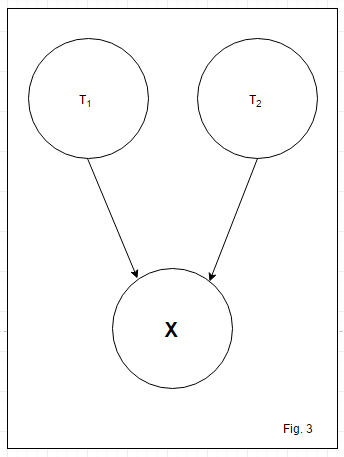
\includegraphics[scale=0.75]{parallel_fig3}\\
     Task dependency diagram of chosen decomposition
\end{figure}

\section{Algorithm Complexity}

\section{OpenMP Implementation}

\end{page}
\end{document}
